\centerline{\bf \huge 10 класс}
\centerline{\bf \huge Решения}

\problem{1}
Верно ли, что любое чётное число, большее 1000, можно представить в виде

$$
n(n+1)(n+2)-m(m+1)
$$


где $m$ и $n$ - натуральные числа?
%Московская область 2017

\textbf{Ответ: Неверно.}
\textbf{Решение.}
Заметим, что произведение трёх последовательных натуральных чисел $n(n+1)(n+$ +2 ) делится на 3 . Разберём несколько случаев.

Если $m$ имеет остаток 0 или 2 при делении на 3 , то $m(m+1)$ делится на 3 . Значит, число $n(n+1)(n+2)-m(m+1)$ делится на 3 .

Если $m$ имеет остаток 1 при делении на 3 , то $m(m+1)$ имеет остаток 2 при делении на 3 . Значит, число $n(n+1)(n+2)-m(m+1)$ имеет остаток 1 при делении на 3 .

Это означает, что число $n(n+1)(n+2)-m(m+1)$ не может иметь остаток 2 при делении на 3. То есть, например, число 1004 в требуемом виде представить не удастся.

\problem{2}
На клетчатой доске $8 \times 8$ размещён 1 клетчатый корабль размера $1 \times 3$. Одним выстрелом разрешается прострелить целиком все 8 клеток одной строки или одного столбца. Какого минимального количества выстрелов хватит, чтобы гарантированно ранить корабль?
%Московская область

\begin{wrapfigure}{r}{0.25\linewidth}
    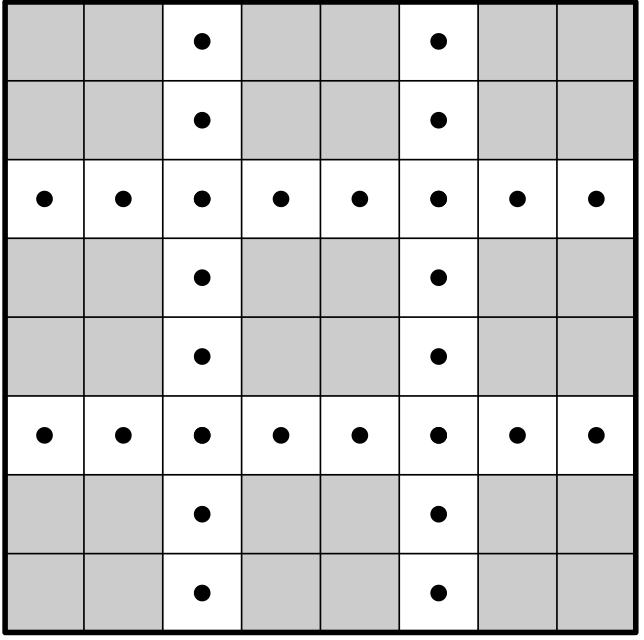
\includegraphics[width=\linewidth]{ЭлМШ 2025-2026/III блок/10/Тренировки/I/Решения/10.2.jpg}
\end{wrapfigure}

\textbf{Ответ: 4 выстрела.}

\textbf{Решение.} Сделаем 4 выстрела так, как показано на рисунке. Тогда видно, что корабль гарантированно будет ранен. Покажем, что если сделано только 3 выстрела, то можно не ранить корабль. Пусть, например, в строки сделано не более одного выстрела. Тогда в любом столбце, в который не сделано выстрела, прострелено не более одной клетки, и поэтому в этом столбце может стоять корабль, который не будет ранен.

\newpage

\hspace{3mm}

\problem{3}
График квадратичной функции $y=a x^2+c$ пересекает оси координат в вершинах правильного треугольника. Чему равно $a c$ ?
%Москва 2017

\textbf{Ответ: -3.}

\textbf{Решение.}
Так как график пересекает ось $O X$ в двух точках, то числа а и с имеют разные знаки. Точки пересечения: $A\left(\sqrt{-\frac{c}{a}} ; 0\right) ; B\left(-\sqrt{-\frac{c}{a}} ; 0\right)$. Ось $OY$ график пересекает в точке $C(0 ; c)$. Тогда сторона $A B$ правильного треугольника равна $2 \sqrt{-\frac{c}{a}}$, а его высота равна $|c|$. Так как сторона а и высота $h$ правильного треугольника связаны соотношением $h=\frac{a \sqrt{3}}{2}$, то $|c|=\frac{\sqrt{3}}{2} \cdot 2 \sqrt{-\frac{c}{a}}$, откуда $c^2=-3 \cdot \frac{c}{a}$, поэтому $a c=-3$.

\problem{4}
Можно ли выбрать число $n \geqslant 3$ и так заполнить таблицу $n \times n$ различными натуральными числами от 1 до $n^2$, чтобы в каждой строке нашлись три числа, одно из которых равно произведению двух других?

\textbf{Ответ: Нельзя.}

\textbf{Решение.}
Предположим, что таблицу удалось заполнить требуемым образом. Рассмотрим в каждой строке три числа: два множителя и их произведение. Отметим в каждой строке наименьший множитель. Так как строк $n$, то всего наименьших множителей $n$. А так как они различны, то среди них найдётся такой, который не меньше $n$. Но тогда в строке, где находится этот множитель, второй множитель будет не меньше $n+1$. Поэтому их произведение не меньше $n(n+1)>n^2$. Противоречие.

\problem{5}
Внутри треугольника $A B C$ отмечена точка $P$. Биссектрисы углов $B A C$ и $A C P$ пересекаются в точке $M$, а биссектриса угла $P B A$ и прямая, содержащая биссектрису угла $B P C$ пересекаются в точке $N$. Докажите, что точка пересечения прямых $C P$ и $A B$ лежит на прямой $MN$.

\textbf{Решение.} 
Пусть прямые $C P$ и $A B$ пересекаются в точке $K$. Тогда $M-$ точка пересечения биссектрис треугольника $A K C$, следовательно, $K M$ --- биссектриса угла $A K C$.

Рассмотрим теперь треугольник $K B P$. $N$ точка пересечения биссектрисы внутреннего угла при вершине $B$ и биссектрисы внешнего угла при вершине $P$. Следовательно, точка $N$ лежит и на биссектрисе внешнего угла при вершине $K$, то есть на биссектрисе угла $A K C$ ($N$ --- центр вневписанной окружности треугольника $K B P)$. Таким образом, точки $K, M$ и N лежат на прямой, содержащей биссектрису угла $AKC$.